%%
%% AG GenomInformatik poster layout
%%
%% Kim Roland Rasmussen
%% September 2004
%%

%%%%%%%%%%%%%%%%%%%%%%%%%%%%%%%%%%%%%%%%%%%%%%%%%%%%%%%%%%%%%%%%%%%%%%%%%%%%%% 
%% Preamble
%%%%%%%%%%%%%%%%%%%%%%%%%%%%%%%%%%%%%%%%%%%%%%%%%%%%%%%%%%%%%%%%%%%%%%%%%%%%%%

\documentclass[portrait]{a0poster}
%\documentclass[portrait,posterdraft]{a0poster}		% Uncomment for draft mode

%% Include packages
\usepackage{a0size}
\usepackage{color}
\usepackage{graphicx}
\usepackage{multicol}
%\usepackage{pstricks}					% Uncomment for PS Tricks
\usepackage{subfigure}
\usepackage{amsmath}
\usepackage{latexsym}
\usepackage[bf]{caption}
\usepackage{sectsty}
\usepackage{verbatim}
\usepackage{aggi}

%% Setup sections font
\allsectionsfont{\sffamily}

%%%%%%%%%%%%%%%%%%%%%%%%%%%%%%%%%%%%%%%%%%%%%%%%%%%%%%%%%%%%%%%%%%%%%%%%%%%%%% 
%% Definitions of title, authors and thanks
%%%%%%%%%%%%%%%%%%%%%%%%%%%%%%%%%%%%%%%%%%%%%%%%%%%%%%%%%%%%%%%%%%%%%%%%%%%%%%

%% You should define \mytitle, \myauthors and \mythanks, each taking one
%% argument.

\mytitle{%
\VERYHuge\bfseries Microarray Layout and the \\
\VERYHuge\bfseries Quadratic Assignment Problem
}

\myauthors{%
\Large\bfseries S\'ergio A. de Carvalho Jr.${}^{1,2,3}$ and Sven Rahmann${}^{2,3}$
}
	
\mythanks{%
\large ${}^1$ Graduiertenkolleg Bioinformatik,
       ${}^2$ International NRW Graduate School in Bioinformatics and Genome Research, \\
\large ${}^3$ Algorithms and Statistics for Systems Biology, Genome Informatics,
              Technische Fakult\"at, Bielefeld University, D-33594 Bielefeld, Germany. \\
\large {\tt \{Sergio.Carvalho, Sven.Rahmann\}@cebitec.uni-bielefeld.de}
}

\newcommand{\ignore}[1]{}
\newcommand{\ds}{\mathcal{S}}

%%%%%%%%%%%%%%%%%%%%%%%%%%%%%%%%%%%%%%%%%%%%%%%%%%%%%%%%%%%%%%%%%%%%%%%%%%%%%% 
%% Misc. document settings
%%%%%%%%%%%%%%%%%%%%%%%%%%%%%%%%%%%%%%%%%%%%%%%%%%%%%%%%%%%%%%%%%%%%%%%%%%%%%%

\begin{document}
\sffamily				% Font used in main text
\large					% Font size used in main text
\setlength{\columnsep}{96pt}		% Width of column separator
\setlength{\columnseprule}{1pt}		% Width of column separator rule
\setlength{\multicolsep}{96pt}		% Space between header and columns

%%%%%%%%%%%%%%%%%%%%%%%%%%%%%%%%%%%%%%%%%%%%%%%%%%%%%%%%%%%%%%%%%%%%%%%%%%%%%% 
%% Header
%%%%%%%%%%%%%%%%%%%%%%%%%%%%%%%%%%%%%%%%%%%%%%%%%%%%%%%%%%%%%%%%%%%%%%%%%%%%%%
\begin{multicols}{3}[\aggiheader]

%%%%%%%%%%%%%%%%%%%%%%%%%%%%%%%%%%%%%%%%%%%%%%%%%%%%%%%%%%%%%%%%%%%%%%%%%%%%%% 
%% Sections
%%%%%%%%%%%%%%%%%%%%%%%%%%%%%%%%%%%%%%%%%%%%%%%%%%%%%%%%%%%%%%%%%%%%%%%%%%%%%%

\setlength{\parskip}{5mm}

\section*{\textcolor{aggigreen}{Introduction}}

\noindent Oligonucleotide microarrays consist of small DNA fragments
(\emph{probes}) chemically synthesized at specific locations (\emph{spots}) on
a coated quartz surface. Probes are typically 25 nt long and are synthesized
in parallel, in a series of repetitive steps. Each step appends a particular
nucleotide to selected regions of the chip. Selection occurs by exposure to
light with the help of a photolithographic mask.

\noindent Formally, we have a set of probes
$\mathcal{P} = \{p_{1}, p_{2}, ... p_{n}\}$ that are produced by a series of
masks $\mathcal{M} = (m_{1}, m_{2}, ... m_T)$, where each mask $m_{t}$ induces
the addition of a particular nucleotide $\ds_{t} \in \{A, C, G, T\}$ to a subset
of~$\mathcal{P}$. The sequence of nucleotides added in each step
$\ds = \ds_{1} \ds_{2} \ldots \ds_{T}$ is called \emph{deposition sequence}.

\noindent In general, a probe can be \emph{embedded} within $\mathcal{S}$ in
several ways. An embedding of $p_k$ is a $T$-tuple
$\varepsilon_{k} = (e_{k,1}, e_{k,2}, ... e_{k,T})$ in which $e_{k,t} = 1$ if
probe $p_{k}$ receives nucleotide $\ds_t$ (at step~$t$), or 0 otherwise
(Figure~\ref{fig:masking_process}).

\begin{myfigure}
\vspace*{4ex}
\centerline{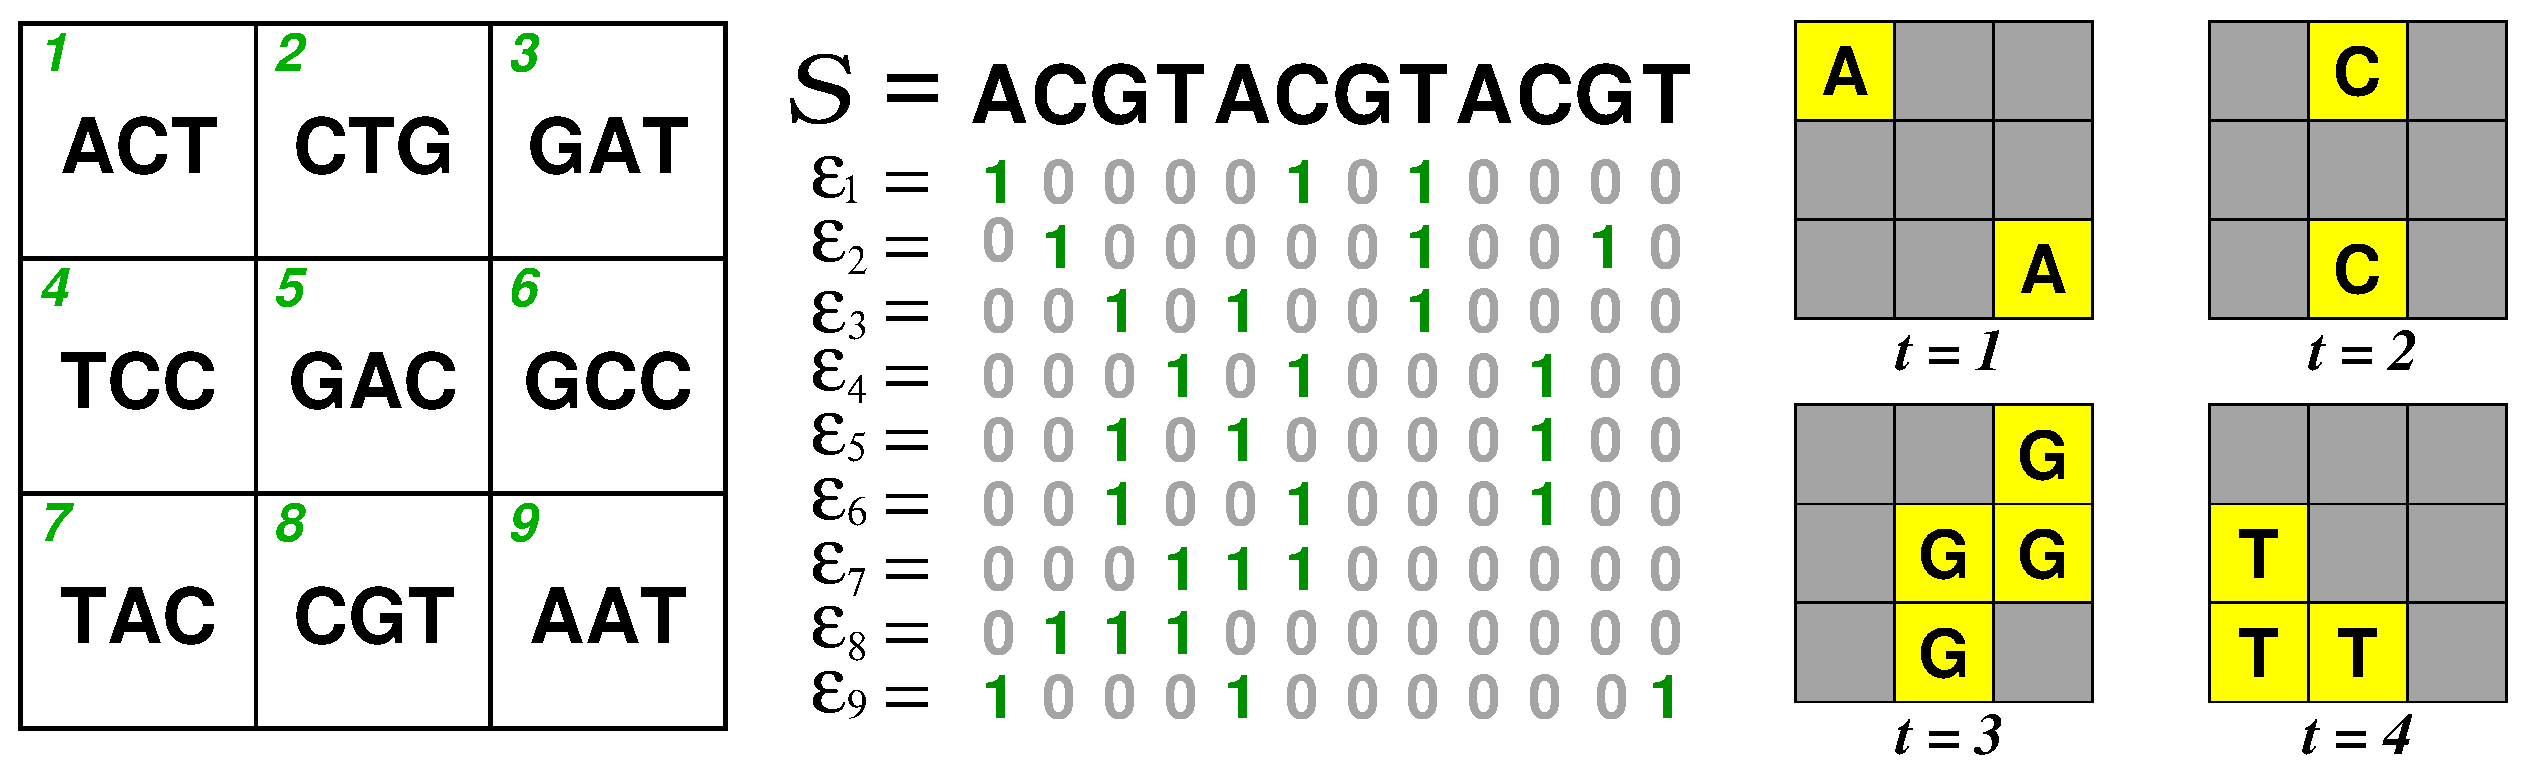
\includegraphics[width=700pt]{chip}}
\caption{Synthesis of a hypothetical 3$\times$3 chip. Left: chip
layout and the 3~nt probe sequences. Center: deposition
sequence and probe embeddings. Right: first four resulting masks.}
\label{fig:masking_process}
\vspace*{4ex}
\end{myfigure}

\noindent Due to diffraction of light or internal reflection, untargeted probes
can be accidentally activated. This is more likely to occur near the borders
between masked and unmasked spots -- hence the term
\textcolor{highlight}{border conflict}.

\subsection*{Border Length}

\noindent The \emph{Border Length Minimization Problem}~\cite{HANNENHALLI02} was
the first formal definition of the problem of unintended illumination. It aims
at finding an arrangement of the probes together with their embeddings with
minimum border conflicts.

\noindent The \emph{border length}~$\mathcal{B}_t$ of mask~$m_{t}$ is defined as
the number of borders shared by masked and unmasked spots at masking step~$t$.
The total border length of a given arrangement is the sum of border lengths over
all masks. The initial four masks shown in Figure~\ref{fig:masking_process} have
$\mathcal{B}_1 = 4$, $\mathcal{B}_2 = 6$, $\mathcal{B}_3 = 6$ and
$\mathcal{B}_4 = 4$. The total border length of that arrangement is 50 (masks 5
to 12 not shown).

\section*{\textcolor{aggigreen}{Conflict Index}}

\noindent We are more interested in estimating the risk of synthesizing a faulty
probe at a given spot. Additionally, two practical considerations need to be
taken into account ~\cite{KAHNG03}:
\begin{itemize}
\item[a)] stray light might activate not only adjacent neighbors but also probes
that lie as far as three cells away from the targeted spot;
\item[b)] imperfections produced in the middle of a probe are more harmful than
in its extremities.
\end{itemize}

\noindent This motivates the following definition of the \emph{conflict
index}~$\mathcal{C}(p)$ of a probe~$p$~\cite{CARVALHO06}. First we define a
distance-dependent weighting function to account for observation a):
%%
\begin{equation}
\label{eq:dist_weight}
\delta(p,p',t) :=
\left\{
        \begin{array}{ll}
                (d(p,p'))^{-2} & \mbox{if $p'$ is unmasked at step $t$}, \\
                0 & \mbox{otherwise}, \\
        \end{array}
\right.
\end{equation}
%%
where $d(p,p')$ is the Euclidean distance between the spots of~$p$ and~$p'$.
We restrict the support of $\delta(p,p',\cdot)$ to those $p'\neq p$ that are in
a $7\times 7$ grid centered around $p$.

\noindent We also define position-dependent weights to account for observation
b):
%%
\begin{equation}\label{eq:pos_mult}
\omega(p,t) :=
\left\{
        \begin{array}{ll}
                c \cdot \exp{\left(\theta \cdot \lambda(p,t)\right)} & \mbox{if $p$ is masked at step $t$}, \\
                0 & \mbox{otherwise}, \\
        \end{array}
\right.
\end{equation}
%%
where $c>0$ and $\theta>0$ are constants (we set $\theta := 5/\ell_p$ and
$c := 1/\exp(\theta)$),
%%
\begin{equation}\label{eq:base_pos}
  \lambda(p,t) := 1 + \min(b_{p,t},\ell_{p} - b_{p,t}),
\end{equation}
%%
$b_{p,t}$ denotes the number of nucleotides synthesized within~$p$ up to and
including step~$t$, and $\ell_{p}$ is the length of probe~$p$.

\noindent We now define the conflict index of a probe $p$ as
\begin{equation}
\label{eq:conf_idx}
\mathcal{C}(p) := \sum_{t=1}^{T} \Bigl( \omega(p,t) \sum_{p'} \delta(p,p',t) \Bigr).
\end{equation}

%% %%%%%%%%%%%%%%%%%%%%%
%% Desired end of column
%% %%%%%%%%%%%%%%%%%%%%%

\section*{\textcolor{aggigreen}{Quadratic Assignment Problem (QAP)}}

\noindent The QAP is a classical combinatorial optimization problem that can be
stated as follows. Given $n \times n$ real-valued matrices $F = (f_{ij})\geq 0$ and $D = (d_{kl})\geq 0$, find a permutation $\pi$ of $\{1, 2, \ldots n\}$ such that
\begin{equation}\label{eq:qap_def}
  \sum_{i=1}^{n} \sum_{j=1}^{n}\,  f_{ij} \cdot d_{\pi(i)\pi(j)} \to \min.
\end{equation}

\noindent One of its major applications is to model the facility location
problem where $n$ facilities are assigned to $n$ locations: $F$ is called
the flow matrix as $f_{ij}$ represents the flow of materials from facility $i$
to facility $j$, while $D$ is called the distance matrix, as $d_{kl}$ gives the
distance between locations $k$ and $l$. The optimal permutation $\pi$ defines a
one-to-one assignment of facilities to locations with minimum cost.

\subsection*{QAP Formulation of Probe Placement}

\noindent The probe placement problem can be seen as an instance of the QAP,
where we want to find a one-to-one correspondence between probes and spots.

\noindent We assume that all probes have a single pre-defined embedding in order
to force a one-to-one relationship (considering all possible embeddings would
still lead to a quadratic integer programming problem). If we have more spots
available than probes to place, we add enough ``empty'' probes and define their
weight functions appropriately.

\noindent Our goal is to design a microarray minimizing the sum of conflict
indices over all probes~$k$, i.e., $\sum_{k} \mathcal{C}(k) \to \min$.

\noindent The ``flow'' $f_{ij}$ between spots $i$ and $j$ depends on their
Euclidean distance $d(i,j)$ on the array:
\begin{equation}
  f_{ij} := \left\{ \begin{array}{ll}
      (d(i,j))^{-2} & \mbox{if spot $j$ is ``near'' spot $i$}, \\
      0 & \mbox{otherwise}. \\
    \end{array} \right.
\end{equation}
%%
where ``near'' means that spot~$j$ is at most three cells away from~$i$. For
Border Length Minimization, we set $f_{ij}:=1$ if spots $i$ and $j$ are direct
neighbors, and $f_{ij}:=0$ otherwise.

\noindent The ``distance'' $d_{kl}$ between probes $k$ and $l$ depends on the
(weighted) Hamming distance of their embeddings. To account for possible
``empty'' probes, we set $d_{kl}:=0$ if $k$ or $l$ or both refer to an empty
probe. Otherwise, we set
\[ d_{kl} := \sum_{t=1}^T\, d_{klt}, \]
where $d_{klt}$ is the potential contribution of probe $l$'s embedding to the
failure risk of probe $p_k$ in the $t$-th synthesis step. According to the
conflict index model,
\[ d_{klt}  = \left\{ \begin{array}{ll}
    c \cdot \exp(\theta \cdot \lambda(p_k,t)) 
    & \mbox{if $p_k$ is masked and $p_l$ unmasked in step $t$,}\\
    0
    & \mbox{otherwise.}
  \end{array} \right.
\]
In the case of Border Length Minimization, where $\theta=0$ and $c=1/2$, we
obtain that $d_{kl} + d_{lk} = H_{kl} = H_{lk}$, where $H_{kl}$ denotes the
Hamming distance between the embeddings of probes $p_k$ and $p_l$.

%% %%%%%%%%%%%%%%%%%%%%%
%% Desired end of column
%% %%%%%%%%%%%%%%%%%%%%%

\section*{\textcolor{aggigreen}{Results}}

\noindent The QAP is known to be NP-hard and particularly hard to solve in
practice. Instances of size larger than $n = 20$ are generally considered to be
impossible to solve to optimality. Nevertheless, our formulation is of interest
because we can now use existing QAP heuristics to design the layout of
microarrays minimizing either the sum of border lengths or conflict indices.

\noindent We used GRASP with path-relinking~\cite{OLIVEIRA04}, a general QAP
heuristic, to design small artificial microarrays, and compared with the
results produced by Row-epitaxial, the best known placement
algorithm~\cite{CARVALHO06} (\ref{tab:graspr_reptx}).

\begin{mytable}
\vspace*{2ex}
\caption{Total border length and average conflict index of chips produced by
Row-epitaxial and GRASP with path-relinking. Reported times in seconds.
\label{tab:graspr_reptx}}
\small{
\begin{tabular}{c||rr|rr||rr|rr|}
     & \multicolumn{4}{|c||}{Border length minimization} & \multicolumn{4}{c|}{Conflict index minimization}                                      \\ \cline{2-9}
     & \multicolumn{2}{|c|}{Row-epitaxial} & \multicolumn{2}{c||}{GRASP-PR} & \multicolumn{2}{c|}{Row-epitaxial} & \multicolumn{2}{c|}{GRASP-PR} \\ \cline{2-9}
Chip & Total     &                          & Total     &                      & Average     &                     & Average  &                  \\
size & b. length & Time                     & b. length & Time                 & c. index    & Time                & c. index & Time             \\ \hline
$6\times 6$   & 1\,714.60 & 0.01 & 1\,672.20 &   2.73 & 495.15 & 0.05 & 467.08 &   3.68 \\
$7\times 7$   & 2\,354.60 & 0.02 & 2\,332.60 &   6.43 & 521.90 & 0.07 & 489.32 &   8.84 \\
$8\times 8$   & 3\,123.80 & 0.03 & 3\,099.13 &  12.49 & 551.84 & 0.09 & 515.69 &  19.48 \\
$9\times 9$   & 3\,974.80 & 0.05 & 3\,967.20 &  25.96 & 568.62 & 0.11 & 533.79 &  38.83 \\
$10\times 10$ & 4\,895.60 & 0.06 & 4\,911.40 &  47.57 & 576.49 & 0.11 & 539.69 &  73.09 \\
$11\times 11$ & 5\,954.40 & 0.10 & 5\,990.73 &  87.48 & 588.91 & 0.12 & 551.41 & 145.67 \\
$12\times 12$ & 7\,086.20 & 0.11 & 7\,159.80 & 152.42 & 598.21 & 0.12 & 561.21 & 249.19 \\ \hline
\end{tabular}}
\vspace*{4ex}
\end{mytable}

Because of the large number of probes on industrial microarrays, it is not
feasible to use a QAP algorithm to design an entire microarray chip, although it
is possible to use it on small sub-regions of a chip. This opens up the way for
two alternatives: 1) combine it with a partitioning algorithm, or 2) use it to
improve an existing layout, iteratively, by relocating probes inside a
sliding-window~\cite{CARVALHO06}.

%%%%%%%%%%%%%%%%%%%%%%%%%%%%%%%%%%%%%%%%%%%%%%%%%%%%%%%%%%%%%%%%%%%%%%%%%%%%%% 
%% Bibliography
%%%%%%%%%%%%%%%%%%%%%%%%%%%%%%%%%%%%%%%%%%%%%%%%%%%%%%%%%%%%%%%%%%%%%%%%%%%%%%
\begin{thebibliography}{9}

\bibitem{HANNENHALLI02} Hannenhalli, S., Hubell, E., Lipshutz, R., Pevzner, P.:
Combinatorial algorithms for design of DNA arrays.
Adv. Biochem. Eng. Biotechnol. {\bfseries77} (2002) 1--19

\bibitem{CARVALHO06}
de Carvalho Jr., S., Rahmann, S.:
Microarray Layout as a Quadratic Assignment Problem.
In {\it German Conference on Bioinformatics (GCB)} (2006), LNI, Springer. To appear.

\bibitem{KAHNG03} Kahng, A. B., Mandoiu, I., Pevzner, P., Reda, S., Zelikovsky, A.:
Engineering a scalable placement heuristic for DNA probe arrays.
Proc. of the Seventh Annual Int. Conf. on Computational Molecular Biology (2003) 148--83

\bibitem{OLIVEIRA04} Oliveira,C.A.S., Pardalos,P.M. and Resende,M.G.C. (2004):
GRASP with path-relinking for the quadratic assignment
problem. In Ribeiro,C.C. and Martins,S.L. (eds.), {\it Efficient and
Experimental Algorithms}, LNCS, {\bf 3059},
356--368, Springer-Verlag.

\end{thebibliography}

\end{multicols}

%%%%%%%%%%%%%%%%%%%%%%%%%%%%%%%%%%%%%%%%%%%%%%%%%%%%%%%%%%%%%%%%%%%%%%%%%%%%%% 
%% Footer
%%%%%%%%%%%%%%%%%%%%%%%%%%%%%%%%%%%%%%%%%%%%%%%%%%%%%%%%%%%%%%%%%%%%%%%%%%%%%%
\aggifooter

\center{Presented at the 14th Annual International Conference on
Intelligent  Systems for Molecular Biology (ISMB), Fortaleza, Brazil,
August 6-10, 2006}

\end{document}
